\chapter{Типы компонентов}

\section{Фотодиоды}

Выбор компонентов для определённого сценария использования определяется требованиями, выдвигаемыми к данной системе. Для фотодиода это может быть: интервал длин волн, которые он может детектировать, скорость отклика, фоточувствительность, сила темнового тока, тип корпуса. Это важно, так как существует значительное количество стандартных компонентов с различными стандартными корпусами, материалами полупроводника, характеристиками. Например, рассмотрим некоторые фотодиоды, представленные на сайте производителя Thorlabs (рисунок~\ref{fig:thorlabs}).

\begin{figure}[!h]
    \centering
    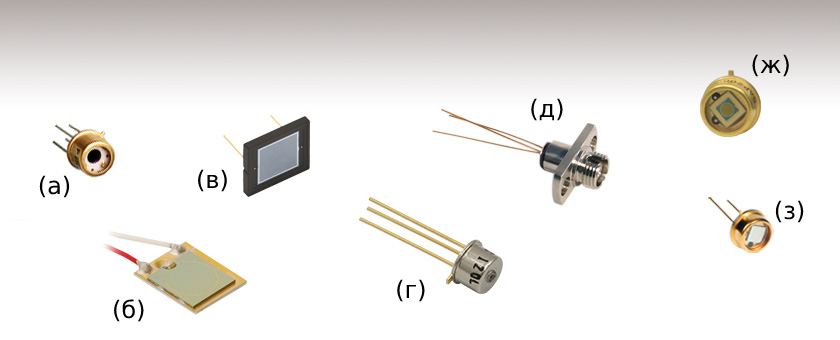
\includegraphics[width=.6\textwidth]{inc/img/thorlabs.png}
    \caption{Некоторые виды полупроводниковых PIN-фотодиодов, представленных на сайте производителя Thorlabs}
    \label{fig:thorlabs}
\end{figure}

\begin{enumerate}
    \item DSD2 \--- двух-зонный фотодиод из Si/InGaAs, кремний находится над InGaAs, за счёт этого фотодиод имеет очень широкий интервал детектируемых длин волн (400\--1100 нм для Si и 1000\--1800 нм для InGaAs), размеры фотодиода: 5.07 мм${}^2$ для Si, 1.77 мм${}^2$ для InGaAs, тип корпуса TO-5;
    \item FDG05 \--- фотодиод из Ge, интервал детектируемых длин волн 800\--1800 нм, размеры фотодиода: 19.6 мм${}^2$, выращен на керамической подложке, поэтому не имеет конкретного типа корпуса;
    \item FDS10X10 \--- большой кремниевый фотодиод с интервалом детектируемых длин волн 340\--1100 нм, с размерами фотодиода 100 мм${}^2$. Аналогично предыдущему выращен на керамической подложке;
    \item FGA01 \--- InGaAs фотодиод с высокой скоростью, типовым корпусом, интервал детектируемых длин волн 800\---1700 нм, размеры фотодиода 0.01 мм${}^2$, имеет стандартный корпус TO-46 и сферическую линзу;
    \item FGA01FC \--- тот же предыдущий фотодиод, но с корпусом, позволяющим подключение к оптоволокну;
    \item FGA21 \--- большой быстрый InGaAs фотодиод с интервалом детектируемых длин волн 800\--1700 нм, размерами фотодиода 3.1 мм${}^2$, тип корпуса TO-5;
    \item FDG03 \--- большой Ge фотодиод в стандартном корпусе TO-5, интервал детектируемых длин волн 800\--1800 нм, размер фотодиода 7.1 мм${}^2$.
\end{enumerate}

\section{Линзы}

Аналогично и для линз существуют различные параметры, которые влияют на характеристики и места применения конкретных линз: габаритные размеры, тип линзы (собирающая/рассеивающая), материал линзы (коэффициент преломления влияет на фокусное расстояние линзы), радиусы кривизны поверхностей (аналогично влияют на фокусное расстояние), толщина линзы по оси, наличие просветляющего покрытия и его материал (наличие покрытия повышает коэффициент пропускания линзы для конкретных длин волн, определяемых материалом покрытия).

Так как для улучшения приёмной части системы есть смысл собирать лучи, падающие на приёмник, была выбрана собирающая линза. Большинство её параметров не имеют значения, так как единственными ограничениями оказываются прозрачный на выбранной длине волны материал и фокусное расстояние, позволяющее разместить активную область фотодиода в фокусе (активная область находится внутри корпуса). Остальные параметры влияют на фокусное расстояние, однако от него будут зависеть габаритные размеры всего приёмного устройство в Li-Fi системе. Исходя из этих ограничений, для моделирования была выбрана выпукло-плоская собирающая линза из оптического стекла К8, прозрачного в ближнем ИК диапазоне. Более подробное описание параметров линзы приведено в разделе~\ref{ch:zemax}.